\documentclass[a4paper, 11pt]{article} % Font size (can be 10pt, 11pt or 12pt) and paper size (remove a4paper for US letter paper)
\textheight=22cm 
\textwidth=15cm 
\topmargin=-1cm 
\oddsidemargin=0cm 

\usepackage[protrusion=true,expansion=true]{microtype} % Better typography
\usepackage{graphicx} % Required for including pictures
\usepackage{wrapfig} % Allows in-line images

\usepackage{mathpazo} % Use the Palatino font
\usepackage[T1]{fontenc} % Required for accented characters
\linespread{1.05} % Change line spacing here, Palatino benefits from a slight increase by default

\makeatletter
\renewcommand\@biblabel[1]{\textbf{#1.}} % Change the square brackets for each bibliography item from '[1]' to '1.'
\renewcommand{\@listI}{\itemsep=0pt} % Reduce the space between items in the itemize and enumerate environments and the bibliography

\renewcommand{\maketitle}{ % Customize the title - do not edit title and author name here, see the TITLE block below
\begin{flushright} % Right align
{\LARGE\@title} % Increase the font size of the title

\vspace{50pt} % Some vertical space between the title and author name

{\large\@author} % Author name
\\\@date % Date

\vspace{40pt} % Some vertical space between the author block and abstract
\end{flushright}
}

%----------------------------------------------------------------------------------------
%	TITLE
%----------------------------------------------------------------------------------------

\title{\textbf{Locating protein-creating genes by parsing DNA sequences with the Viterbi algorithm}\\ % Title
\vspace{0.5cm}
{\Large Stochastic Models and Optimization Project}} % Subtitle

\author{\textbf{Roger Cusc\'o, Matthew Sudmann-Day and Miquel Torrens} % Author
\vspace{0.1cm}
\\{{\large \textit{Barcelona Graduate School of Economics}}}} % Institution


\date{\vspace{0.5cm} {\large April 1, 2016}} % Date

%----------------------------------------------------------------------------------------

\begin{document}

\maketitle % Print the title section

%----------------------------------------------------------------------------------------
%	ABSTRACT AND KEYWORDS
%----------------------------------------------------------------------------------------

%\renewcommand{\abstractname}{Summary} % Uncomment to change the name of the abstract to something else

\begin{abstract}
Pure data-driven algorithms are becoming increasingly important in genomics. One important application of their use is that of determining which parts of the DNA are used in the creation of certain proteins, which is a task that cannot always be determined in the decoding stage. In this project, we use DNA sequences to apply the Viterbi algorithm with hidden Markov models so as to predict which sequences are relevant in the process of synthesising proteins. The algorithm developed is able to correctly classify about three fourths of the newly observed DNA sequences and predict whether they are useful in the protein creation process.
\end{abstract}

\hspace*{3,6mm}\textit{Keywords:} genomics, dynamic programming, hidden Markov, Viterbi algorithm % Keywords

\vspace{30pt} % Some vertical space between the abstract and first section

%----------------------------------------------------------------------------------------
%	ESSAY BODY
%----------------------------------------------------------------------------------------

\section*{Framework}

The DNA is a molecule in the core of each organic cell that contains all the information needed to develop a living organism. Yet, its structure is surprisingly simple. It essentially boils down to a long sequence of joint molecules \textendash called nucleotides$-$ structured in the shape of a double helix. The sequence consists of only four different nucleotides, permutated in different patterns that will later determine which proteins will be synthetised. These four nucleotides are usually denoted by the following four letters: \texttt{A} (adenine), \texttt{G} (guanine), \texttt{C} (cytosine) and \texttt{T} (thymine), the four nucleobases. DNA sequencing is the process of translating a DNA molecule into a sequence of \texttt{A}, \texttt{G}, \texttt{C} and \texttt{T}'s, which gives rise to the different molecular combinations that originate distinct proteins. These will be the backbone for the survival of the organism.

In the biological process of translating DNA into proteins, the sequence of corresponding nucleotides, e.g. \texttt{ACTTCCGTA...}, is first translated into aminoacids, which will then participate in the creation of proteins. One aminoacid is the result of reading a sequence of three nucleotides, known as a codon. There are 64 possible codons, each of which has its properties\footnote{An example: \texttt{ACT} is the Threonine.}.

\begin{wrapfigure}{l}{0.4\textwidth} % Inline image example
\begin{center}
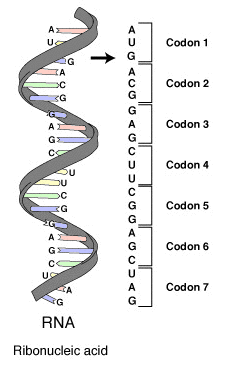
\includegraphics[width=0.38\textwidth]{rna_codons.png}
\end{center}
\caption{An RNA sequence.}
\end{wrapfigure}

The reading process is performed by an RNA messenger, which is a molecule almost identical to the DNA\footnote{The difference between the two lies in the fact that the RNA has an extra atom of oxigen in its molecular structure.}. This messenger will match its own sequence with the one in the DNA and carry the relevant information encoded in the subsequence extracted for protein creation to the ribosome, another part of the cell. There, the subsequence is read and the final protein is produced, using the aminoacids carried on the RNA. The unique sequence matched for each protein corresponds to a known gene.

%------------------------------------------------

\section*{The Challenge}

Given the extraordinary length of the DNA sequence in complex organisms\footnote{A human chromosome can have up to 500 million base pairs of DNA with thousands of genes.}, detecting what parts of of the sequence are actually used and what are their purposes is not a trivial task to perform. Modern genomics delve into finding relations between subsequences of the RNA and the posterior protein created. This is the well-known gene finding problem. To tackle this task, one of the most important objectives is to locate where these subparts start and end, as most of the DNA sequence does not have a known biological use.

Our goal in this project is to identify those regions of the DNA that are used in the synthesis of proteins. In other words, we look for patterns that signal the beginning or the end of such regions. The detection of relevant regions in the DNA is an active field of research, as it helps understand, for instance, the origin of certain genetic diseases, as in \cite{scheper} or \cite{calon}, among many other examples.

The combination of a Hidden Markov Model (HMM) and the well-known dynamic programming Viterbi algorithm have been commonly used in the last two decades to help in that task (see for example \cite{henderson}).

%------------------------------------------------
\section*{Methodology}

Hidden Markov models and dynamic programming have been used in the past for the detection of used subsequences, known as exons, and unused ones, known as introns. 

To carry out this task, we make use of the Molecular Biology Splice-junction Gene Sequences Dataset\footnote{Available publicly at: \texttt{http://bit.ly/25yuniW} \cite{lichman}.}, from the UCI Machine Learning repository, and then apply our particular implementation of a HMM and an adapted Viterbi algorithm to find these regions in this dataset.

The dataset consists of 3,190 short sequences of DNA extracted from mammals, each of which contains a string of 60 base nucleotides. We illustrate an example of such 60-character sequences:
\begin{eqnarray}
\texttt{CCAGCTGCATCACAGGAGGCCAGCGAGCAGGTCTGTTCCAAGGGCCTTCGAGCCAGTCTG}  \nonumber
\end{eqnarray}
Each of these sequences is labeled as an exon region (\texttt{EI}), intron region (\texttt{IE}) or neither (\texttt{N}). The sample is unbalanced towards regions labeled as \texttt{N}, with approximately half of the observations. Exon and intron regions represent roughly 25\% of the sample each. From now on, for consistency with the terminology of our model, we are going to refer to the labels as states and to the nucleotides as symbols. A sequence of five symbols will be called an observation, also known in some contexts as poly-codon. We have chosen to define the observations as combinations of symbols to account for the fact that nucleotides do not translate directly into proteins. As mentioned earlier, they have to be translated into amino acids first, which are composed by strings of three nucleotides. However, here we include additional nucleotides in our unit measure of observation. This is done to maximize the accuracy of the model, as more complex observations can be expected to better capture the particular patterns found in an exon or intron.

Thus, we have:
\begin{itemize}
\item Symbols: \texttt{A}, \texttt{C}, \texttt{G}, \texttt{T}
\item Observations: \texttt{AAAAA}, ..., \texttt{AGTCT}, ..., \texttt{TTTTT}. A total of $4^5=1024$ distinct values.
\item States: \texttt{EI}, \texttt{IE}, \texttt{N}.
\end{itemize}

Our model has to infer the state of each sequence from its string of 60 symbols. To do so, we first set up an HMM using the a priori and conditional probabilities inferred from the dataset with the following parameters:
\begin{itemize}
\item  $\mathbb{P}(x_0) \equiv \mathbb{P}(x_0 = x_{k})$, where $x_{k} \in \{\texttt{EI}, \texttt{IE}, \texttt{N} \}$, is a vector of initial probabilities for each of the states. The sub-index $k$ refers to element $k$ on the list of possible states.
\item $\mathbb{P}(x_i | x_{i-1}) \equiv \mathbb{P}(x_i = x_k | x_{i-1})$, where $x_{i}, x_{k} \in \{\texttt{EI}, \texttt{IE}, \texttt{N} \}$, which are the transition probabilities of changing from state $i-1$ to state $i$. Sub-index $i$ refers to the position in the string.
%\item $a(x_{i}, x_{j})$ where $x_{i}, x_{j} \in \{\texttt{EI}, \texttt{IE}, \texttt{N} \}$, which is the transition matrix indicating the probability of changing from state $i$ to state $j$.
\item $\mathbb{P}(z_i | x_i, x_{i-1}) \equiv \mathbb{P}(z_i = z_l | x_i, x_{i-1})$ where $x_{i} \in \{\texttt{EI}, \texttt{IE}, \texttt{N} \}$ and $z_i, z_{l} \in \{\texttt{AAAAA}, \dots, \texttt{TTTTT}\}$, which represent the emission probabilities of producing symbol $z_{i}$ when transitioning from state $x_{i-1}$ to state $x_{i}$. Sub-index $l$ refers to the list of possible five-letter substrings of the DNA.
\end{itemize}

Once the HMM is trained, we need to find the most likely sequence of hidden states that has generated any given sequence of symbols. To do that, we use a Viterbi algorithm.

Given a sequence of observations $\textbf{z} = \{ z_{1},..., z_{n} \}$, where $n$ is the length of the sequence, we want to estimate the most likely path of states $\textbf{x}^V = \{ x_{1}^V, ..., x_{n}^V \}$, that has been generated by $\textbf{z}$. The true path $\textbf{x} = \{ x_{1}, ..., x_{n} \}$ is unknown. In other words, we want to find the path of states that maximizes the conditional probability $\mathbb{P}(\textbf{x} | \textbf{z})$, which can also be rewritten as $\mathbb{P}(\textbf{x},\textbf{z})/\mathbb{P}(\textbf{z})$. Since $\mathbb{P}(\textbf{z})$ is a positive constant, because $\textbf{z}$ is known, we can just maximise the joint probability, that results in $\textbf{x}^V$. Therefore:
\begin{eqnarray}
\mathbb{P}(\textbf{x}, \textbf{z}) &=& \mathbb{P}(x_{0},...,x_{n},z_{1},...,z_{n})  \nonumber \\
&=& \mathbb{P}(x_{0})\mathbb{P}(x_{1},...,x_{n},z_{1},...,z_{n} | x_{0}).  \nonumber
\end{eqnarray}
Applying recursively the law of total probability we get:
\begin{eqnarray}
\mathbb{P}(\textbf{x}, \textbf{z}) &=& \mathbb{P}(x_{0}) \prod^{N}_{i=1} \mathbb{P}(z_i | x_i, x_{i-1}) \mathbb{P}(x_i | x_{i-1}).   \nonumber
\end{eqnarray}
Using a logarithmic transformation, we can express our problem as:
\begin{eqnarray}
\min_{x_0, x_1, \dots, x_N} \left[ -\log \mathbb{P}(x_{0}) - \sum^{N}_{k=1} \left( \log \mathbb{P}(z_i | x_i, x_{i-1}) + \log \mathbb{P}(x_i | x_{i-1}) \right) \right],  \nonumber
\end{eqnarray}
Taking a closer look at the nature of the problem, we see that it can be represented as a shortest path problem, where the shortest path will be the sequence of states that minimizes the negative likelihood expressed above.

\begin{wrapfigure}{r}{0.6\textwidth} % Inline image example
\begin{center}
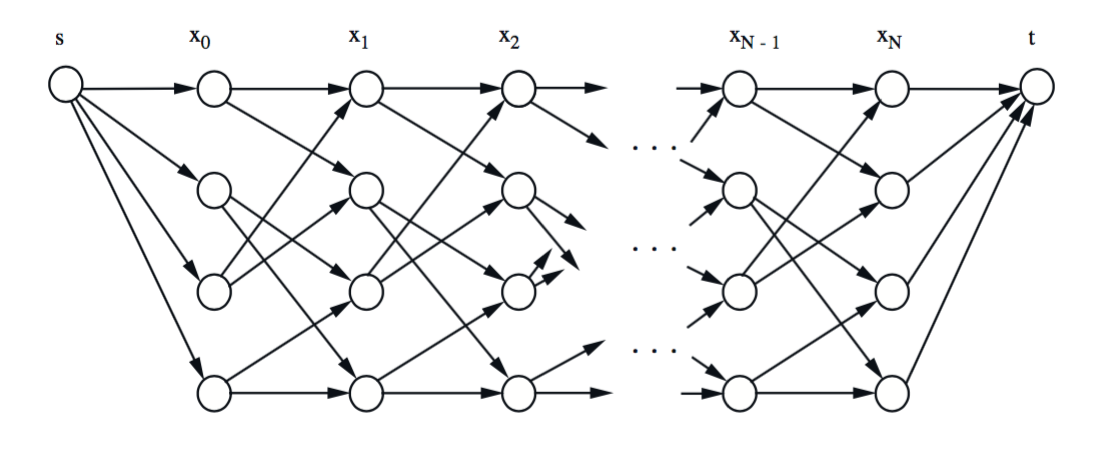
\includegraphics[width=0.58\textwidth]{trellis.png}
\end{center}
\caption{Viterbi trellis.}
\end{wrapfigure}

The trellis diagram for such a minimum path problem would look as in Figure 2, where the edges from $s$ to $x_{0}$ have weight $-\log \mathbb{P}(x_{0})$, the edges from $x_{N}$ to $t$ have weight 0, and any edge from $x_{i-1}$ to $x_{i}$ has a corresponding weight $-\left( \log \mathbb{P}(x_{i}|x_{i-1} + \log \mathbb{P}(z_{i}|x_{i}, x_{i-1})) \right)$. The path that minimises the sum of all the weights would be our estimated sequence of states $\textbf{x}^V = \{ x_{1}^V, ..., x_N^V \}$.

As the cost \textendash in this case, weight$-$ of every edge is known, there is no noise or disturbance to account for, and the problem can be solved with forward DP. In our case, the algorithm would be initialized with $D_{0}(x_{0}) = -\log \mathbb{P}(x_{0})$ and proceed as follows:

\begin{eqnarray}
D_{i}(x_{i}) = \min_{ x_i: \mathbb{P}(x_i | x_{i-1}) > 0} \left[ D_{i-1}(x_{i-1}) - \left( \log \mathbb{P}(z_i | x_i, x_{i-1}) + \log \mathbb{P}(x_i | x_{i-1}) \right) \right],  \nonumber
\end{eqnarray}

for $i \in \{ 1, \dots, N \}$. This is known as the Viterbi algorithm.

On top of the regular Viterbi algorithm described above, we had to implement an extra step due to the fixed length of our sequences. Unlike the classical Viterbi algorithm, that returns a sequence of states or transitions from an observed sequence of symbols, we had to group the sequence of predicted states into a single prediction every 60 symbols. This is due to the construction of the dataset. 

We have sequences of DNA of 60 nucleotides, which translate into 12 observations, and each of the sequences has a common state. All of the observations in a sequence are labeled as either \texttt{EI}, \texttt{IE} or \texttt{N} in our dataset. Consequently, the path of states predicted by the Viterbi algorithm must be mapped into a sequence 12 times shorter. To do that, we have evaluated the posterior probabilities for every state at each iteration an taken the state with the highest average posterior probability in a given sequence of 12 observations.

Previous to that, the set of sequences had to be ordered as the data set did not contain the sequences with their true succession. To do that, we simulated the order of the set using the values of the prior probabilities and restricting the Markov Chain by the genomic construction of the DNA, meaning restricting by what is and is not allowed to follow each state, always respecting the total class frequencies.

We have coded\footnote{The full code can be found in: \texttt{https://github.com/mtorrens/dna}.} the described Viterbi algorithm in \texttt{R}. 

%------------------------------------------------
\section*{Results}

In order to improve the results a bit, the Viterbi algorithm is run both forward and backwards within a sequence. If both directions coincide in classification (vast majority of the times), then the label is clear. If they differ, the one with highest posterior probability is applied. This has been conducted due to the heavy weight imposed by the first observed subsequence.

Three different amounts of subsequences have been attempted: 3 letters (codon level), 5 (poly-codon) and 6 (di-codon). We kept five letters as it maximised the cross-validation scores at all levels. To validate the model, $k$-fold cross-validation is performed, as well as leave-one-out error. Using the entire set for training, we achieved in-sample success rate of 82.4\%, that is broken down with 83.8\% correct labels in the exon regions, 78.4\% in the intron regions and 83.5\% in the regions that are neither.

Cross-validation scores are a bit weaker but still remarkable. Five-fold cross-validation obtains 71.2\% success rate, ten-fold obtains 71.0\%, hundred-fold gets to 72.5\%. Leave-one-out cross-validation, the most unbiased estimator, hits 73.0\% of the labels correctly. The model is able to score with almost the same accuracy intron-exon, exon-intron and neither regions.

There is a reason reason behind the difference between the cross-validation scores. When the algorithm finds in the test stage a sequence that it had not observed in the training set, it is not able to compute the posterior probability. In such case, our model assigns the highest prior probability. Given that the number of combinations in five characters is reasonably finite, as we increase the training set, the number of unobserved subsequences tends rapidly to zero, which allows the leave-one-out error estimate to outstand. Its algorithm is trained with the largest amount of distinct combinations and, thus, is able to compute posterior probabilities for virtually all sequences.

%------------------------------------------------


%------------------------------------------------
\section*{Conclusions}

Modern genomics have introduced new sequencing methodologies, empowered by the increasing computational power when processing large chunks of DNA data. Neural networks have achieved identification success rates well above 90\%. Nonetheless, this example has proven that this approach is simple, comprehensible, decently powerful and not too computationally intensive. It is an algorithm that is not as data-hungry as its neural networks counterpart. This combination of hidden Markov models and the Viterbi algorithm was a state-of-the-art innovative technique that achieved an outstanding success rate at its discovery.

Additionally, some characteristics of particular sub-problems tied to the decoding of the DNA still make the HMM and Viterbi approach a top-class research technique, as modern research uses this method with different objectives, see for example \cite{schreiber} or \cite{sacher}. Hopefully, the increasing amount of processed and sequenced information will allow this methodology to be powerful and widely used in an increasing amount of advanced genomics research.

%----------------------------------------------------------------------------------------
%	BIBLIOGRAPHY
%----------------------------------------------------------------------------------------

\medskip
\bibliographystyle{unsrt}

\begin{thebibliography}{9}

\bibitem{bertsekas}
Bertsekas, D.P. (1996).
\textit{Dynamic Programming and Optimal Control} (Vol. I, 3rd Edition). ISBNs: 1-886529-26-4.

\bibitem{calon}
Calon, A. et al. (2012).
\textit{Dependency of Colorectal Cancer on a TGF-$\beta$-Driven Program in Stromal Cells for Metastasis Initiation}.
Cancer Cell, Volume 22, Issue 5, 571-584.

\bibitem{henderson}
Henderson, J., Salzberg, S. and Fasman, K.H. (1997).
\textit{Finding Genes in DNA with a Hidden Markov Model}.
Journal of Computational Biology, 1997 Summer; 4(2):127-41.

\bibitem{lichman}
Lichman, M. (2013).
\textit{UCI Machine Learning Repository} [http://archive.ics.uci.edu/ml]. Irvine, CA: University of California, School of Information and Computer Science.

\bibitem{scheper}
Scheper, G.C., van der Knaap, M.S. and Proud, C.G. (2007).
\textit{Translation matters: protein synthesis defects in inherited disease}.
Nature Reviews Genetics, 2007 Sep; 8(9):711-23.

\bibitem{schreiber}
Schreiber, J. and Karplus, K. (2015).
\textit{Analysis of Nanopore Data using Hidden Markov Models}.
Bioinformatics, 2015 Jun 15; 31(12):1897-903.

\bibitem{sramek}
\v{S}r\'amek, R., Brejov\'a, B. and Vina\v{r}, T. (2007)
\textit{On-line Viterbi Algorithm for Analysis of Long Biological Sequences}.
Algorithms in Bioinformatics: 7th International Workshop (WABI), 4645 volume of Lecture Notes in Computer Science, pp. 240-251, Philadelphia, PA, USA.

\bibitem{zacher}
Zacher, B. et al. (2014).
\textit{Annotation of genomics data using bidirectional hidden Markov models unveils variations in Pol II transcription cycle}.
Molecular Systems Biology, 2014 Dec; 10(12):768. 

\end{thebibliography}
%----------------------------------------------------------------------------------------

\end{document}